\chapter{Introduction}\label{chap:intro}
During the course of this year, I will be undertaking a project, which to my hope shall be up to standard of a level eight degree in software and development. Initially I was given the option to be assigned a group, or to work on my own. I have chosen to work by myself, as I feel I can assign myself a good level of scope for the project required. Additionally, I did not wish to be assigned into a group as I had done group work in the past, which worked well however, I never had a say in the application my team was making, this made it really hard to gel into the team, as some design choices were not feasible with too much scope taken into the project. I feel if I operate by myself I can make good design choices and which can be reflected in my project. At the start of the year I coined with working on a project in unity, for example a 3d shooter, with a simple AI of enemies to come and find the player around a medium sized map. However after some thought I imagined the scope would have been too big for one person to take on. My next idea was to create a MERN(Mongo, Express, React, Node) \cite{mern}, CRUD(Create, Read, Update, Delete) \cite{crud} application, to upload memories in a social app setting. This application would also showcase new skills I wished to take on such as testing using cypress, which is a JavaScript testing tool to automatically simulate user behaviour such as button clicks. I decided this application would best suits my skills, as I can engage with new technologies in particular, automated testing. I decided to call the application Echo, I felt this was a unique name as it means to be reminiscent of the past, in which users of the application, may post memories or adventures of their past.

\section{My Idea}\label{section:idea}
My intention is to create a MERN stack application to compliment cypress test automation, with a sign in/register system, sending messages to other users, uploading pictures, liking, and commenting on pictures. In conjuncture to have a fully automated test suite set up using cypress, test cases will also be created to accompany and structure the JavaScript code in cypress, test cases are instructions on how the program should be used, simulating behaviour of a user. My hope is to create a friendly environment where users can upload their travels around the world with friends, or cool hobbies. In addition showcasing new technology for example cypress, in which test automation is used to reduce time from manually testing. Below is a wire frame of how I wish the application to look.

\begin{figure}[h!]
    \centering
    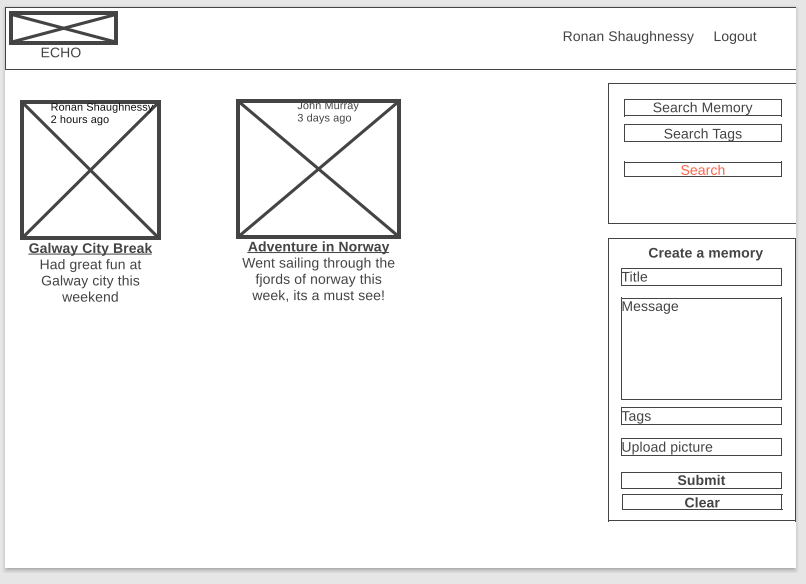
\includegraphics[width=0.78\textwidth]{images/WireFrame.png}
    \caption{Application Homepage.}
    \label{image:AppHome}
\end{figure}

\section{Technology Stack}\label{section:stack}
I plan to use a variety of programming languages I have acquired during the last three years for instance, HTML, CSS, JavaScript, and TypeScript. I decided on MongoDB for my database as according to research I conducted, it stores records as documents, combined with mongoose it can create documents for storing pictures, or any other storage the user will need. I opted for MongoDB over MySQL as I used MySQL often over the last three years, and I wished for a new challenge. I wanted to design the structure of my documents with MongoDB as I find it easier to change Mongo's schema compared to MySQL. I will connect my front-end and back-end using express.js, node.js. Lastly, I will use React for my front-end. I picked React over Angular as during my research I found that React is better for larger web applications as it is more light weight, and I can develop quicker. I feel angular's framework is more rigid and strict combined with the fact React is used more in 2022. Additionally, I wish to improve my skills in software testing, to this end I will employ cypress automated testing to complete testing automatically using TypeScript, and cucumber. Cypress with the aid of TypeScript can create scripts which simulate button clicks, routing to pages etc. This will make testing faster, improving my skills in software testing. I have chosen cypress over selenium as I have never covered cypress, to give me a new challenge and to automate my tests. Following research, I found that cypress manages execution time performance more efficiently than selenium, cypress uses less source lines of code(SLOC) and looks neater when reviewing test cases in the browser \cite{cypresssel}.

\section{Objectives}\label{section:objectives}
The paramount goal is to develop a single-page application, dynamically updating the application, which then allows the user to display photos of their memories and adventures. Moreover to create an application which simulates user behaviour such as button clicks automatically. In order to reach this goal, the subsequent objectives must be present in the application.
\begin{itemize}
    \item To create a dynamic single page application.
    \item The user can register their own account with the application.
    \item The user can sign into their own account once     	registered.
    \item A user is able to post pictures, they wish to share with their friends/family.
    \item Users can search for certain memories using taglines or memory titles.
    \item Users can send messages between each other.
    \item A user is allowed to like a picture, and comment underneath it.
    \item Users can create bio's underneath their posts.
    \item Users should be able to login to their profile and logout.
    \item Designing test scenarios to use in conjunction with cypress automated test tool. 
    \item To have a fully automated test features to verify    the application for commercial use, using test case scenarios designed.
\end{itemize}

\section{Aims}
The purpose of creating the application, what I expect to achieve during the development of the website.
\begin{itemize}
    \item To build a highly pleasing front-end website, which will have a great appearance to please all who visit the application.
    \item To create multiple test scenarios, and have such scenarios fully automated using cypress.
    \item To improve my website design skills using React and JavaScript.
    \item To further my ability using automated testing.
\end{itemize}

\section{Overview}
A brief description of the chapters in this dissertation which illustrate the rationale behind designing this project.
\subsection{Methodology}
This segment describes the work undertaken during the development stage, with particular emphasis on approach to development, validation, testing and tools used to aid development.
\subsection{Technology Review}
This section outlines the technologies which were used in this project, setting up the aforementioned technologies and how the technologies were applied throughout the project.
\subsection{System Design}
This chapter will detail how the project was assembled, how the back-end interacts with the front-end, and will provide a comprehensive description of the overall system architecture.
\subsection{System Evaluation}
This segment will evaluate if the project met the objectives listed in the introduction, and discuss how effectively the system was implemented.
\subsection{Conclusion}
The last chapter examines if the objectives arrayed in the introduction chapter were met, trials which occurred during the development of the project, and how such difficulties were overcome.
\subsection{GitHub Repository}
The GitHub repository for ECHO, my final year project can be found by clicking \href{https://github.com/Rshocks/Final-Year-Project}here.
